\let\negmedspace\undefined
\let\negthickspace\undefined
\documentclass[journal]{IEEEtran}
\usepackage[a5paper, margin=10mm, onecolumn]{geometry}
\usepackage{lmodern} % Ensure lmodern is loaded for pdflatex
\usepackage{tfrupee} % Include tfrupee package

\setlength{\headheight}{1cm} % Set the height of the header box
\setlength{\headsep}{0mm}     % Set the distance between the header box and the top of the text

\usepackage{gvv-book}
\usepackage{gvv}
\usepackage{cite}
\usepackage{amsmath,amssymb,amsfonts,amsthm}
\usepackage{algorithmic}
\usepackage{graphicx}
\usepackage{textcomp}
\usepackage{xcolor}
\usepackage{txfonts}
\usepackage{listings}
\usepackage{enumitem}
\usepackage{mathtools}
\usepackage{gensymb}
\usepackage{comment}
\usepackage[breaklinks=true]{hyperref}
\usepackage{tkz-euclide} 
\usepackage{listings}
\usepackage{gvv}                                        
\def\inputGnumericTable{}                                 
\usepackage[latin1]{inputenc}                                
\usepackage{color}                                            
\usepackage{array}                                            
\usepackage{longtable}                                       
\usepackage{calc}                                             
\usepackage{multirow}                                         
\usepackage{hhline}                                           
\usepackage{ifthen}                                           
\usepackage{lscape}
\begin{document}

\bibliographystyle{IEEEtran}
\vspace{3cm}

\title{12.8.1.8}
\author{EE24BTECH11060-Sruthi bijili}
% \maketitle
% \newpage
% \bigskip
{\let\newpage\relax\maketitle}
\textbf{Question:}\\
Prove that the area between $x = y^2$ and $x = 4$ is divided into two equal parts by the line $x = \frac{8}{3}$\\
\textbf{Solution:}\\
The equation of parabola is $g \brak{\vec{x}} = \vec{x}^{\top}\vec{V}\vec{x} + 2 \vec{u}^{\top}\vec{x} + f = 0$. In matrix form, it is given by,
\begin{align}
	\myvec{x & y} \myvec{0 & 0 \\ 0 & 1} \myvec{x \\ y} + 2 \myvec{-\frac{1}{2} & 0} \myvec{x \\ y} + 0 = 0
\end{align}
Line equation is,
\begin{align}
	\vec{x} = \kappa \myvec{0\\1} + \myvec{4\\0}
\end{align}
Intersection of a line and a conic is given by,
\begin{align}
	\kappa_i = \frac{-\vec{m}^{\top}\brak{\vec{Vh}+\vec{u}}\pm\sqrt{\sbrak{\vec{m}^{\top}\brak{\vec{Vh}+\vec{u}}}^2-g\brak{h}\brak{\vec{m}^{\top}\vec{Vm}}}}{\vec{m}^{\top}\vec{Vm}}
\end{align}
For the given conic, $\vec{V}=\myvec{0 & 0 \\ 0 & 1 }, \vec{u} = \myvec{-\frac{1}{2}\\ 0}, f = 0$. For the given line, $\vec{h}=\myvec{4 \\ 0}$, $\vec{m}=\myvec{0 \\ 1}$
\begin{multline}
     k_i =\frac{1}{\myvec{0 
 & 1}\myvec{0 &0  \\ 0 & 1}\myvec{0 \\ 1}}\brak{-\myvec{0&1}\brak{\myvec{0&0\\0&1}\myvec{4\\0}+\myvec{-\frac{1}{2}\\0}}}\pm \\
     \sqrt{\sbrak{\myvec{0&1}\brak{\myvec{0&0\\0&1}\myvec{4\\0}+\myvec{-\frac{1}{2}\\0}}}^2-g\brak{h}\brak{\myvec{0&1}\myvec{0&0\\0&1}\myvec{0\\1}}} 
\end{multline}
by the solving the equation we get
\begin{align}	
	\implies \kappa_i = \myvec{ 4\\2} , \myvec{4\\ -2}
\end{align}
The 2 curves meet at the points \myvec{2\\4} and \myvec{-1\\ 1}. So, the area between the curves is given by,\\
By using the above formula for the line $x=\frac{8}{3}$ we get\\
\begin{align}	
	\implies \kappa=\myvec{\frac{8}{3} \\ \frac{2\sqrt{6}}{3}}, \myvec{\frac{8}{3} \\ -\frac{2\sqrt{6}}{3}}
\end{align}
\textbf{Theoretical Solution:}\\
Area between $x=4$ and $x=y^2$
\begin{align}
	\int{\brak{4 - y^2}}dy
    \implies \sbrak{4y}_{-2}^{2} -\sbrak{\frac{y^3}{3}}_{-2}^{2}\\
	\implies \brak{16} - \brak{\frac{16}{3}}\\
	\implies \frac{32}{3} sq.units
\end{align}
Area between $x=\frac{8}{3}$ and $x=y^2$
\begin{align}
	\int{\brak{\frac{8}{3} - y^2}}dy\\
	\implies \sbrak{\frac{8}{3}y}_{-\frac{2\sqrt{6}}{3}}^{\frac{2\sqrt{6}}{3}} - \sbrak{\frac{y^3}{3}}_{-\frac{2\sqrt{6}}{3}}^{\frac{2\sqrt{6}}{3}}\\
	\implies \frac{16}{3} sq.units
\end{align}
The first area is twice than the second area. Thus,the line $x=\frac{8}{3}$ divides the area into two equal parts.\\   
\textbf{Simulated Solution:}\\
Using the Trapezoidal rule which approximates the ntegral of a function $f\brak{x}$ over an interval $\sbrak{a,b}$ by dividing the interval into $n$ subintervals and approximating the area under the curve as a series of trapezoids
\begin{align}
    \int_a^b f\brak{x}dx\approx\frac{h}{2}\sbrak{f\brak{x_0}+2\sum_{i=1}^{n-1}\brak{f\brak{x_i}+f\brak{x_n}}}
\end{align}
Where $x_0$ is semi-major axis of ellipse and $x_n$ is semi-minor axis of the ellipse and $h$ is the width of each subinterval.
\begin{align}
    x_n=x_0+n\cdot h\\
    \implies h=\frac{x_n-x_0}{n}
\end{align}
Let $A\brak{x_n}$ be the area enclosed by the curve $y\brak{x}$ from $x=x_0$ to $x=x_n$, $\brak{x_0, x_1, \dots x_n}$ be equidistant points with step-size $h$. Then,
\begin{align}
  A\brak{x_n+h}=A\brak{x_n}+\frac{1}{2}h\brak{y\brak{x_n+h}+y\brak{x_n}}
\end{align}
where $\frac{1}{2}h\brak{y\brak{x_n+h}+y\brak{x_n}}$ is area of difference trapezium
We can repeat this till we get the required area.\\
Let $A(x_n)=A_n$ and $y(x_n)=y_n$
\begin{align}
        A_{n+1}=A_n+\frac{1}{2}h\brak{y_{n+1}+y_n}
\end{align}
We can write $y_{n+1}$ in terms of $y_n$ using first principle of derivative. $y_{n+1}=y_n+hy^{\prime}_n$
\begin{align}
  A_{n+1}&=A_n+\frac{1}{2}h\brak{\brak{y_{n}+hy^{\prime}_n}+y_n}\\
  A_{n+1}&=A_n+\frac{1}{2}h\brak{2y_n+hy^{\prime}_n}\\
  A_{n+1}&=A_n+hy_n+\frac{1}{2}h^2y^{\prime}_n\label{2}\\
\end{align}
In the given question, $y^2=x$ and $y^{\prime}=\frac{1}{2\sqrt{x}}$\newline
General Difference Equation is given by, from \ref{2}
\begin{align}
  A_{n+1}&=A_n+hy_n+\frac{1}{2}h^2y^{\prime}_n\\
  &=A_n+h\brak{\sqrt{x_n}}+\frac{1}{2}h^2\brak{\frac{1}{2\sqrt{x_n}}}\\
  x_{n+1}&=x_n+h
\end{align}
By iterating through the required value of $n$, we get the area enclosed between the line and the parabola.\\
Theoretical area $= \frac{32}{3}$ sq.units\\
Calculated area through trapezoidal rule $=10.6667$ sq.units\\

Below is the plot for line and the parabola
\begin{figure}[h!]
	\centering
	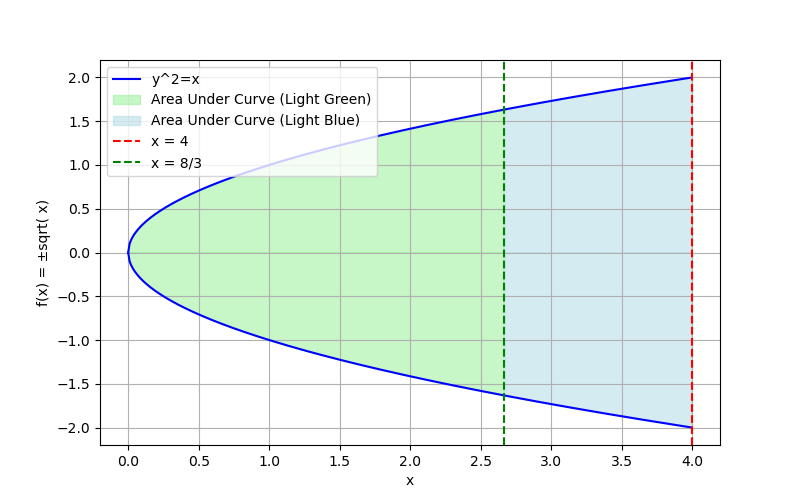
\includegraphics[width=1\columnwidth]{figs/fig.png}
	\label{stemplot}
\end{figure}






\end{document}
